\documentclass[1p]{elsarticle_modified}
%\bibliographystyle{elsarticle-num}

%\usepackage[colorlinks]{hyperref}
%\usepackage{abbrmath_seonhwa} %\Abb, \Ascr, \Acal ,\Abf, \Afrak
\usepackage{amsfonts}
\usepackage{amssymb}
\usepackage{amsmath}
\usepackage{amsthm}
\usepackage{scalefnt}
\usepackage{amsbsy}
\usepackage{kotex}
\usepackage{caption}
\usepackage{subfig}
\usepackage{color}
\usepackage{graphicx}
\usepackage{xcolor} %% white, black, red, green, blue, cyan, magenta, yellow
\usepackage{float}
\usepackage{setspace}
\usepackage{hyperref}

\usepackage{tikz}
\usetikzlibrary{arrows}

\usepackage{multirow}
\usepackage{array} % fixed length table
\usepackage{hhline}

%%%%%%%%%%%%%%%%%%%%%
\makeatletter
\renewcommand*\env@matrix[1][\arraystretch]{%
	\edef\arraystretch{#1}%
	\hskip -\arraycolsep
	\let\@ifnextchar\new@ifnextchar
	\array{*\c@MaxMatrixCols c}}
\makeatother %https://tex.stackexchange.com/questions/14071/how-can-i-increase-the-line-spacing-in-a-matrix
%%%%%%%%%%%%%%%

\usepackage[normalem]{ulem}

\newcommand{\msout}[1]{\ifmmode\text{\sout{\ensuremath{#1}}}\else\sout{#1}\fi}
%SOURCE: \msout is \stkout macro in https://tex.stackexchange.com/questions/20609/strikeout-in-math-mode

\newcommand{\cancel}[1]{
	\ifmmode
	{\color{red}\msout{#1}}
	\else
	{\color{red}\sout{#1}}
	\fi
}

\newcommand{\add}[1]{
	{\color{blue}\uwave{#1}}
}

\newcommand{\replace}[2]{
	\ifmmode
	{\color{red}\msout{#1}}{\color{blue}\uwave{#2}}
	\else
	{\color{red}\sout{#1}}{\color{blue}\uwave{#2}}
	\fi
}

\newcommand{\Sol}{\mathcal{S}} %segment
\newcommand{\D}{D} %diagram
\newcommand{\A}{\mathcal{A}} %arc


%%%%%%%%%%%%%%%%%%%%%%%%%%%%%5 test

\def\sl{\operatorname{\textup{SL}}(2,\Cbb)}
\def\psl{\operatorname{\textup{PSL}}(2,\Cbb)}
\def\quan{\mkern 1mu \triangleright \mkern 1mu}

\theoremstyle{definition}
\newtheorem{thm}{Theorem}[section]
\newtheorem{prop}[thm]{Proposition}
\newtheorem{lem}[thm]{Lemma}
\newtheorem{ques}[thm]{Question}
\newtheorem{cor}[thm]{Corollary}
\newtheorem{defn}[thm]{Definition}
\newtheorem{exam}[thm]{Example}
\newtheorem{rmk}[thm]{Remark}
\newtheorem{alg}[thm]{Algorithm}

\newcommand{\I}{\sqrt{-1}}
\begin{document}

%\begin{frontmatter}
%
%\title{Boundary parabolic representations of knots up to 8 crossings}
%
%%% Group authors per affiliation:
%\author{Yunhi Cho} 
%\address{Department of Mathematics, University of Seoul, Seoul, Korea}
%\ead{yhcho@uos.ac.kr}
%
%
%\author{Seonhwa Kim} %\fnref{s_kim}}
%\address{Center for Geometry and Physics, Institute for Basic Science, Pohang, 37673, Korea}
%\ead{ryeona17@ibs.re.kr}
%
%\author{Hyuk Kim}
%\address{Department of Mathematical Sciences, Seoul National University, Seoul 08826, Korea}
%\ead{hyukkim@snu.ac.kr}
%
%\author{Seokbeom Yoon}
%\address{Department of Mathematical Sciences, Seoul National University, Seoul, 08826,  Korea}
%\ead{sbyoon15@snu.ac.kr}
%
%\begin{abstract}
%We find all boundary parabolic representation of knots up to 8 crossings.
%
%\end{abstract}
%\begin{keyword}
%    \MSC[2010] 57M25 
%\end{keyword}
%
%\end{frontmatter}

%\linenumbers
%\tableofcontents
%
\newcommand\colored[1]{\textcolor{white}{\rule[-0.35ex]{0.8em}{1.4ex}}\kern-0.8em\color{red} #1}%
%\newcommand\colored[1]{\textcolor{white}{ #1}\kern-2.17ex	\textcolor{white}{ #1}\kern-1.81ex	\textcolor{white}{ #1}\kern-2.15ex\color{red}#1	}

{\Large $\underline{12a_{0065}~(K12a_{0065})}$}

\setlength{\tabcolsep}{10pt}
\renewcommand{\arraystretch}{1.6}
\vspace{1cm}\begin{tabular}{m{100pt}>{\centering\arraybackslash}m{274pt}}
\multirow{5}{120pt}{
	\centering
	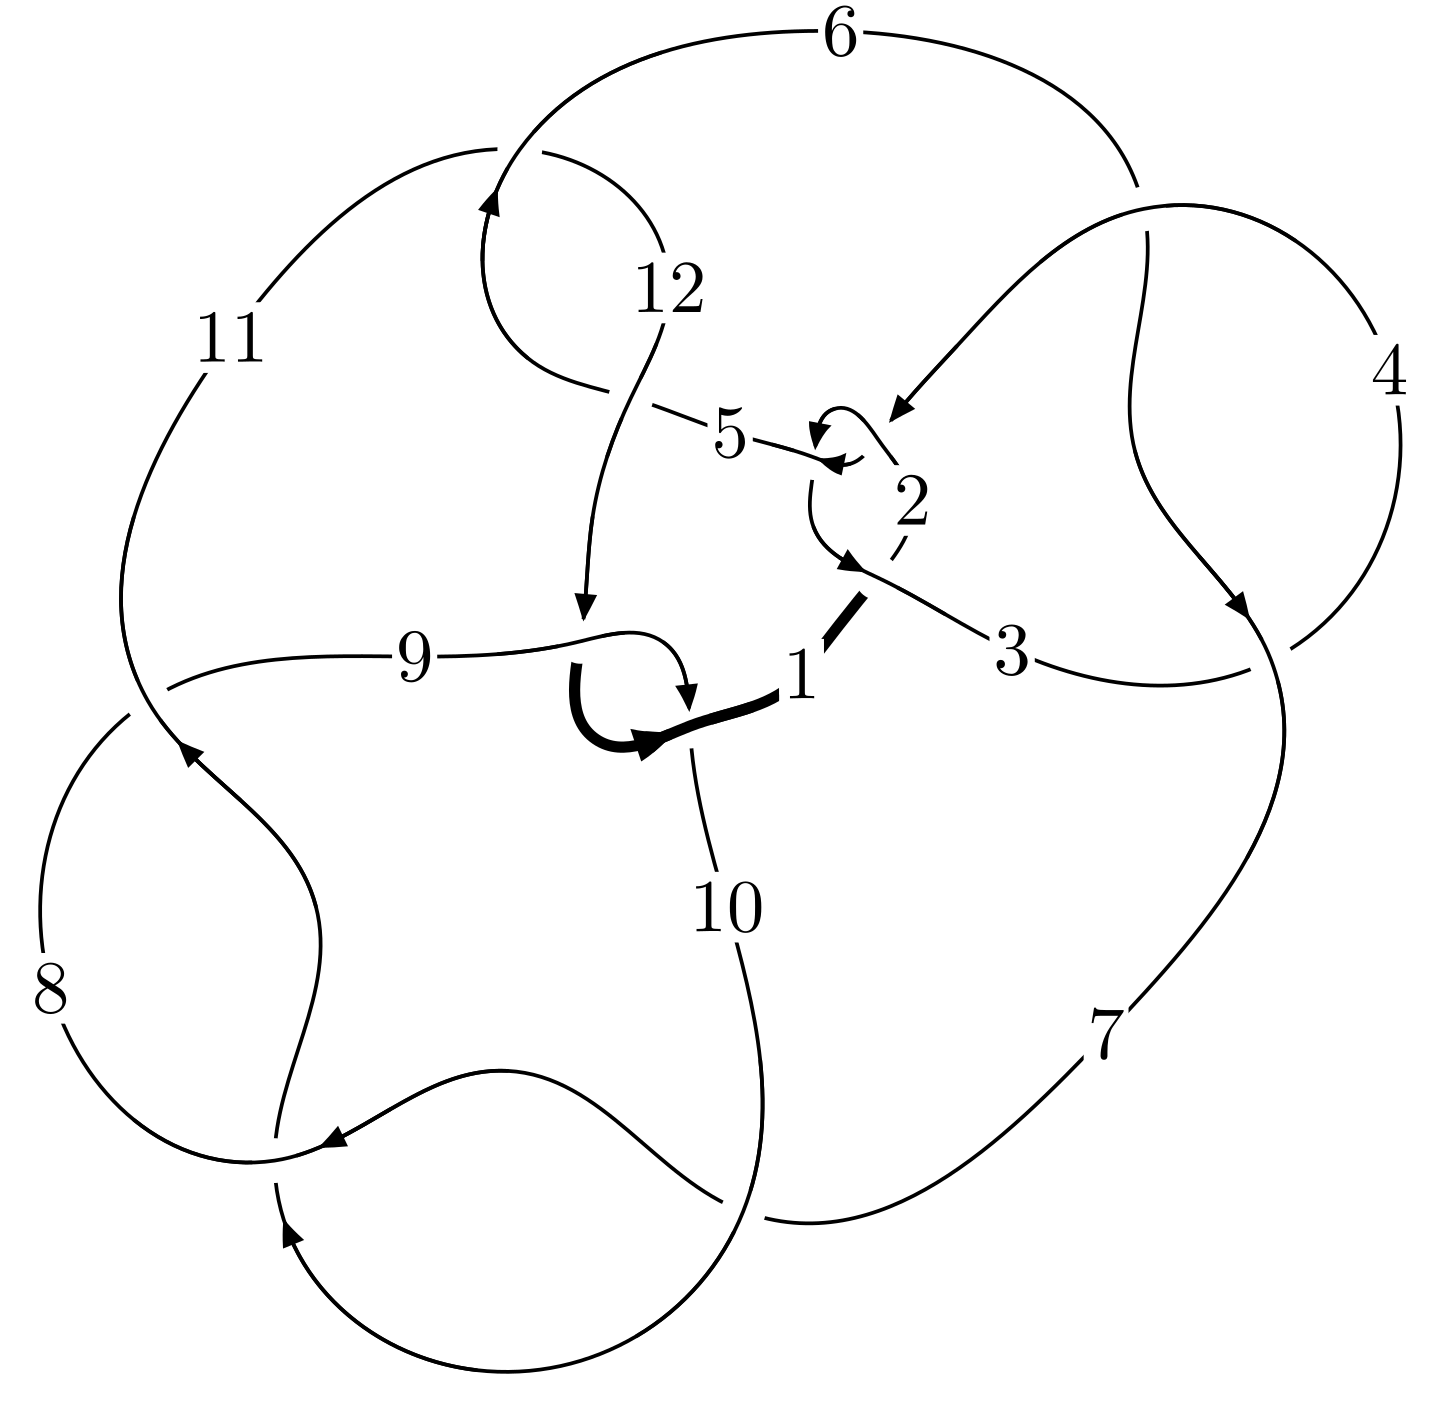
\includegraphics[width=112pt]{../../../GIT/diagram.site/Diagrams/png/866_12a_0065.png}\\
\ \ \ A knot diagram\footnotemark}&
\allowdisplaybreaks
\textbf{Linearized knot diagam} \\
\cline{2-2}
 &
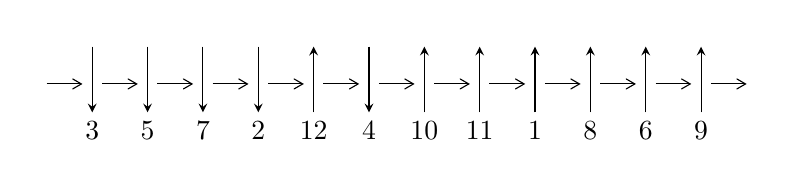
\begin{tikzpicture}[x=20pt, y=17pt]
	% nodes
	\node (C0) at (0, 0) {};
	\node (C1) at (1, 0) {};
	\node (C1U) at (1, +1) {};
	\node (C1D) at (1, -1) {3};

	\node (C2) at (2, 0) {};
	\node (C2U) at (2, +1) {};
	\node (C2D) at (2, -1) {5};

	\node (C3) at (3, 0) {};
	\node (C3U) at (3, +1) {};
	\node (C3D) at (3, -1) {7};

	\node (C4) at (4, 0) {};
	\node (C4U) at (4, +1) {};
	\node (C4D) at (4, -1) {2};

	\node (C5) at (5, 0) {};
	\node (C5U) at (5, +1) {};
	\node (C5D) at (5, -1) {12};

	\node (C6) at (6, 0) {};
	\node (C6U) at (6, +1) {};
	\node (C6D) at (6, -1) {4};

	\node (C7) at (7, 0) {};
	\node (C7U) at (7, +1) {};
	\node (C7D) at (7, -1) {10};

	\node (C8) at (8, 0) {};
	\node (C8U) at (8, +1) {};
	\node (C8D) at (8, -1) {11};

	\node (C9) at (9, 0) {};
	\node (C9U) at (9, +1) {};
	\node (C9D) at (9, -1) {1};

	\node (C10) at (10, 0) {};
	\node (C10U) at (10, +1) {};
	\node (C10D) at (10, -1) {8};

	\node (C11) at (11, 0) {};
	\node (C11U) at (11, +1) {};
	\node (C11D) at (11, -1) {6};

	\node (C12) at (12, 0) {};
	\node (C12U) at (12, +1) {};
	\node (C12D) at (12, -1) {9};
	\node (C13) at (13, 0) {};

	% arrows
	\draw[->,>={angle 60}]
	(C0) edge (C1) (C1) edge (C2) (C2) edge (C3) (C3) edge (C4) (C4) edge (C5) (C5) edge (C6) (C6) edge (C7) (C7) edge (C8) (C8) edge (C9) (C9) edge (C10) (C10) edge (C11) (C11) edge (C12) (C12) edge (C13) ;	\draw[->,>=stealth]
	(C1U) edge (C1D) (C2U) edge (C2D) (C3U) edge (C3D) (C4U) edge (C4D) (C5D) edge (C5U) (C6U) edge (C6D) (C7D) edge (C7U) (C8D) edge (C8U) (C9D) edge (C9U) (C10D) edge (C10U) (C11D) edge (C11U) (C12D) edge (C12U) ;
	\end{tikzpicture} \\
\hhline{~~} \\& 
\textbf{Solving Sequence} \\ \cline{2-2} 
 &
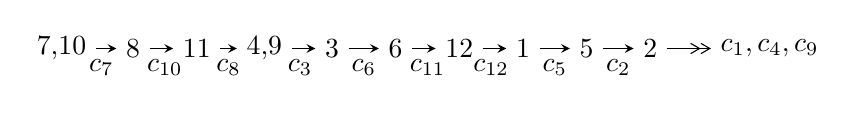
\begin{tikzpicture}[x=23pt, y=7pt]
	% node
	\node (A0) at (-1/8, 0) {7,10};
	\node (A1) at (1, 0) {8};
	\node (A2) at (2, 0) {11};
	\node (A3) at (49/16, 0) {4,9};
	\node (A4) at (33/8, 0) {3};
	\node (A5) at (41/8, 0) {6};
	\node (A6) at (49/8, 0) {12};
	\node (A7) at (57/8, 0) {1};
	\node (A8) at (65/8, 0) {5};
	\node (A9) at (73/8, 0) {2};
	\node (C1) at (1/2, -1) {$c_{7}$};
	\node (C2) at (3/2, -1) {$c_{10}$};
	\node (C3) at (5/2, -1) {$c_{8}$};
	\node (C4) at (29/8, -1) {$c_{3}$};
	\node (C5) at (37/8, -1) {$c_{6}$};
	\node (C6) at (45/8, -1) {$c_{11}$};
	\node (C7) at (53/8, -1) {$c_{12}$};
	\node (C8) at (61/8, -1) {$c_{5}$};
	\node (C9) at (69/8, -1) {$c_{2}$};
	\node (A10) at (11, 0) {$c_{1},c_{4},c_{9}$};

	% edge
	\draw[->,>=stealth]	
	(A0) edge (A1) (A1) edge (A2) (A2) edge (A3) (A3) edge (A4) (A4) edge (A5) (A5) edge (A6) (A6) edge (A7) (A7) edge (A8) (A8) edge (A9) ;
	\draw[->>,>={angle 60}]	
	(A9) edge (A10);
\end{tikzpicture} \\ 

\end{tabular} \\

\footnotetext{
The image of knot diagram is generated by the software ``\textbf{Draw programme}" developed by Andrew Bartholomew(\url{http://www.layer8.co.uk/maths/draw/index.htm\#Running-draw}), where we modified some parts for our purpose(\url{https://github.com/CATsTAILs/LinksPainter}).
}\phantom \\ \newline 
\centering \textbf{Ideals for irreducible components\footnotemark of $X_{\text{par}}$} 
 
\begin{align*}
I^u_{1}&=\langle 
-2.92249\times10^{169} u^{111}+3.73944\times10^{170} u^{110}+\cdots+1.17142\times10^{167} b-2.38948\times10^{169},\\
\phantom{I^u_{1}}&\phantom{= \langle  }-4.45166\times10^{168} u^{111}+5.26012\times10^{169} u^{110}+\cdots+5.85711\times10^{166} a-7.08065\times10^{168},\\
\phantom{I^u_{1}}&\phantom{= \langle  }u^{112}-14 u^{111}+\cdots-171 u-1\rangle \\
I^u_{2}&=\langle 
313 a^8+2651 a^7-1632 a^6+9330 a^5-4960 a^4+9676 a^3-3659 a^2+145 b+3312 a-888,\\
\phantom{I^u_{2}}&\phantom{= \langle  }a^9+8 a^8-9 a^7+34 a^6-30 a^5+42 a^4-26 a^3+17 a^2-7 a+1,\;u+1\rangle \\
I^u_{3}&=\langle 
b,\;3 u^7-5 u^6-7 u^5+11 u^4+5 u^3-3 u^2+a-7,\;u^8- u^7-3 u^6+2 u^5+3 u^4-2 u-1\rangle \\
I^u_{4}&=\langle 
3 a^2 u- a^2+10 a u+11 b-7 a+9 u-3,\;a^3- a^2 u+3 a^2- a u+4 a- u+5,\;u^2- u-1\rangle \\
\\
\end{align*}
\raggedright * 4 irreducible components of $\dim_{\mathbb{C}}=0$, with total 135 representations.\\
\footnotetext{All coefficients of polynomials are rational numbers. But the coefficients are sometimes approximated in decimal forms when there is not enough margin.}
\newpage
\renewcommand{\arraystretch}{1}
\centering \section*{I. $I^u_{1}= \langle -2.92\times10^{169} u^{111}+3.74\times10^{170} u^{110}+\cdots+1.17\times10^{167} b-2.39\times10^{169},\;-4.45\times10^{168} u^{111}+5.26\times10^{169} u^{110}+\cdots+5.86\times10^{166} a-7.08\times10^{168},\;u^{112}-14 u^{111}+\cdots-171 u-1 \rangle$}
\flushleft \textbf{(i) Arc colorings}\\
\begin{tabular}{m{7pt} m{180pt} m{7pt} m{180pt} }
\flushright $a_{7}=$&$\begin{pmatrix}1\\0\end{pmatrix}$ \\
\flushright $a_{10}=$&$\begin{pmatrix}0\\u\end{pmatrix}$ \\
\flushright $a_{8}=$&$\begin{pmatrix}1\\- u^2\end{pmatrix}$ \\
\flushright $a_{11}=$&$\begin{pmatrix}u\\- u^3+u\end{pmatrix}$ \\
\flushright $a_{4}=$&$\begin{pmatrix}76.0044 u^{111}-898.076 u^{110}+\cdots+4341.78 u+120.890\\249.483 u^{111}-3192.23 u^{110}+\cdots+34958.2 u+203.982\end{pmatrix}$ \\
\flushright $a_{9}=$&$\begin{pmatrix}- u^2+1\\u^4-2 u^2\end{pmatrix}$ \\
\flushright $a_{3}=$&$\begin{pmatrix}325.487 u^{111}-4090.30 u^{110}+\cdots+39300.0 u+324.872\\249.483 u^{111}-3192.23 u^{110}+\cdots+34958.2 u+203.982\end{pmatrix}$ \\
\flushright $a_{6}=$&$\begin{pmatrix}-323.912 u^{111}+4095.13 u^{110}+\cdots-41394.8 u-288.132\\684.638 u^{111}-8698.30 u^{110}+\cdots+90947.7 u+529.205\end{pmatrix}$ \\
\flushright $a_{12}=$&$\begin{pmatrix}17.9543 u^{111}-189.370 u^{110}+\cdots-880.998 u-18.0322\\72.8595 u^{111}-925.927 u^{110}+\cdots+8953.79 u+52.0848\end{pmatrix}$ \\
\flushright $a_{1}=$&$\begin{pmatrix}196.977 u^{111}-2493.83 u^{110}+\cdots+24770.7 u+131.202\\311.051 u^{111}-3876.48 u^{110}+\cdots+33723.8 u+196.443\end{pmatrix}$ \\
\flushright $a_{5}=$&$\begin{pmatrix}-270.582 u^{111}+3459.45 u^{110}+\cdots-38028.8 u-272.024\\-248.530 u^{111}+3130.15 u^{110}+\cdots-30299.4 u-176.735\end{pmatrix}$ \\
\flushright $a_{2}=$&$\begin{pmatrix}49.6326 u^{111}-561.615 u^{110}+\cdots-239.766 u+52.4969\\248.530 u^{111}-3130.15 u^{110}+\cdots+30299.4 u+176.735\end{pmatrix}$\\&\end{tabular}
\flushleft \textbf{(ii) Obstruction class $= -1$}\\~\\
\flushleft \textbf{(iii) Cusp Shapes $= -360.979 u^{111}+4669.85 u^{110}+\cdots-55646.3 u-332.781$}\\~\\
\newpage\renewcommand{\arraystretch}{1}
\flushleft \textbf{(iv) u-Polynomials at the component}\newline \\
\begin{tabular}{m{50pt}|m{274pt}}
Crossings & \hspace{64pt}u-Polynomials at each crossing \\
\hline $$\begin{aligned}c_{1}\end{aligned}$$&$\begin{aligned}
&u^{112}+52 u^{111}+\cdots+6550 u+1
\end{aligned}$\\
\hline $$\begin{aligned}c_{2},c_{4}\end{aligned}$$&$\begin{aligned}
&u^{112}-12 u^{111}+\cdots+78 u+1
\end{aligned}$\\
\hline $$\begin{aligned}c_{3},c_{6}\end{aligned}$$&$\begin{aligned}
&u^{112}-4 u^{111}+\cdots-1664 u+256
\end{aligned}$\\
\hline $$\begin{aligned}c_{5},c_{11}\end{aligned}$$&$\begin{aligned}
&u^{112}+3 u^{111}+\cdots-224 u-64
\end{aligned}$\\
\hline $$\begin{aligned}c_{7},c_{8},c_{10}\end{aligned}$$&$\begin{aligned}
&u^{112}+14 u^{111}+\cdots+171 u-1
\end{aligned}$\\
\hline $$\begin{aligned}c_{9},c_{12}\end{aligned}$$&$\begin{aligned}
&u^{112}-5 u^{111}+\cdots-5632 u+512
\end{aligned}$\\
\hline
\end{tabular}\\~\\
\newpage\renewcommand{\arraystretch}{1}
\flushleft \textbf{(v) Riley Polynomials at the component}\newline \\
\begin{tabular}{m{50pt}|m{274pt}}
Crossings & \hspace{64pt}Riley Polynomials at each crossing \\
\hline $$\begin{aligned}c_{1}\end{aligned}$$&$\begin{aligned}
&y^{112}+28 y^{111}+\cdots-43105022 y+1
\end{aligned}$\\
\hline $$\begin{aligned}c_{2},c_{4}\end{aligned}$$&$\begin{aligned}
&y^{112}-52 y^{111}+\cdots-6550 y+1
\end{aligned}$\\
\hline $$\begin{aligned}c_{3},c_{6}\end{aligned}$$&$\begin{aligned}
&y^{112}+60 y^{111}+\cdots-3784704 y+65536
\end{aligned}$\\
\hline $$\begin{aligned}c_{5},c_{11}\end{aligned}$$&$\begin{aligned}
&y^{112}+47 y^{111}+\cdots-185344 y+4096
\end{aligned}$\\
\hline $$\begin{aligned}c_{7},c_{8},c_{10}\end{aligned}$$&$\begin{aligned}
&y^{112}-110 y^{111}+\cdots-28983 y+1
\end{aligned}$\\
\hline $$\begin{aligned}c_{9},c_{12}\end{aligned}$$&$\begin{aligned}
&y^{112}-69 y^{111}+\cdots-75235328 y+262144
\end{aligned}$\\
\hline
\end{tabular}\\~\\
\newpage\flushleft \textbf{(vi) Complex Volumes and Cusp Shapes}
$$\begin{array}{c|c|c}  
\text{Solutions to }I^u_{1}& \I (\text{vol} + \sqrt{-1}CS) & \text{Cusp shape}\\
 \hline 
\begin{aligned}
u &= -0.432227 + 0.899551 I \\
a &= \phantom{-}0.863303 - 0.682893 I \\
b &= \phantom{-}0.503098 + 1.270930 I\end{aligned}
 & \phantom{-}3.43374 - 7.46948 I & \phantom{-0.000000 } 0 \\ \hline\begin{aligned}
u &= -0.432227 - 0.899551 I \\
a &= \phantom{-}0.863303 + 0.682893 I \\
b &= \phantom{-}0.503098 - 1.270930 I\end{aligned}
 & \phantom{-}3.43374 + 7.46948 I & \phantom{-0.000000 } 0 \\ \hline\begin{aligned}
u &= -0.994475\phantom{ +0.000000I} \\
a &= \phantom{-}10.9938\phantom{ +0.000000I} \\
b &= \phantom{-}0.530791\phantom{ +0.000000I}\end{aligned}
 & \phantom{-}0.460815\phantom{ +0.000000I} & \phantom{-0.000000 } 0 \\ \hline\begin{aligned}
u &= -0.807871 + 0.613058 I \\
a &= -0.88505 + 1.10731 I \\
b &= -0.906023 - 0.341572 I\end{aligned}
 & -0.13349 + 1.76727 I & \phantom{-0.000000 } 0 \\ \hline\begin{aligned}
u &= -0.807871 - 0.613058 I \\
a &= -0.88505 - 1.10731 I \\
b &= -0.906023 + 0.341572 I\end{aligned}
 & -0.13349 - 1.76727 I & \phantom{-0.000000 } 0 \\ \hline\begin{aligned}
u &= -0.397239 + 0.960530 I \\
a &= -1.051620 + 0.624722 I \\
b &= -0.68926 - 1.24272 I\end{aligned}
 & \phantom{-}1.11481 - 13.24070 I & \phantom{-0.000000 } 0 \\ \hline\begin{aligned}
u &= -0.397239 - 0.960530 I \\
a &= -1.051620 - 0.624722 I \\
b &= -0.68926 + 1.24272 I\end{aligned}
 & \phantom{-}1.11481 + 13.24070 I & \phantom{-0.000000 } 0 \\ \hline\begin{aligned}
u &= -0.846216 + 0.417781 I \\
a &= \phantom{-}0.01284 - 2.09013 I \\
b &= -0.291691 + 0.590527 I\end{aligned}
 & -0.994600 - 0.244702 I & \phantom{-0.000000 } 0 \\ \hline\begin{aligned}
u &= -0.846216 - 0.417781 I \\
a &= \phantom{-}0.01284 + 2.09013 I \\
b &= -0.291691 - 0.590527 I\end{aligned}
 & -0.994600 + 0.244702 I & \phantom{-0.000000 } 0 \\ \hline\begin{aligned}
u &= -0.371874 + 0.847663 I \\
a &= -0.637100 + 0.223721 I \\
b &= -1.082290 + 0.424589 I\end{aligned}
 & -1.50046 - 6.83730 I & \phantom{-0.000000 } 0\\
 \hline 
 \end{array}$$\newpage$$\begin{array}{c|c|c}  
\text{Solutions to }I^u_{1}& \I (\text{vol} + \sqrt{-1}CS) & \text{Cusp shape}\\
 \hline 
\begin{aligned}
u &= -0.371874 - 0.847663 I \\
a &= -0.637100 - 0.223721 I \\
b &= -1.082290 - 0.424589 I\end{aligned}
 & -1.50046 + 6.83730 I & \phantom{-0.000000 } 0 \\ \hline\begin{aligned}
u &= -1.063340 + 0.200741 I \\
a &= -0.591192 - 0.953846 I \\
b &= \phantom{-}0.378594 + 0.254527 I\end{aligned}
 & \phantom{-}1.19166 - 0.82959 I & \phantom{-0.000000 } 0 \\ \hline\begin{aligned}
u &= -1.063340 - 0.200741 I \\
a &= -0.591192 + 0.953846 I \\
b &= \phantom{-}0.378594 - 0.254527 I\end{aligned}
 & \phantom{-}1.19166 + 0.82959 I & \phantom{-0.000000 } 0 \\ \hline\begin{aligned}
u &= -0.784572 + 0.755080 I \\
a &= -0.521418 + 0.547316 I \\
b &= \phantom{-}0.363354 - 1.200850 I\end{aligned}
 & \phantom{-}4.50061 + 1.87825 I & \phantom{-0.000000 } 0 \\ \hline\begin{aligned}
u &= -0.784572 - 0.755080 I \\
a &= -0.521418 - 0.547316 I \\
b &= \phantom{-}0.363354 + 1.200850 I\end{aligned}
 & \phantom{-}4.50061 - 1.87825 I & \phantom{-0.000000 } 0 \\ \hline\begin{aligned}
u &= -0.471032 + 0.748109 I \\
a &= -1.383900 + 0.286927 I \\
b &= -0.298324 - 1.206400 I\end{aligned}
 & \phantom{-}4.78310 - 1.56650 I & \phantom{-0.000000 } 0 \\ \hline\begin{aligned}
u &= -0.471032 - 0.748109 I \\
a &= -1.383900 - 0.286927 I \\
b &= -0.298324 + 1.206400 I\end{aligned}
 & \phantom{-}4.78310 + 1.56650 I & \phantom{-0.000000 } 0 \\ \hline\begin{aligned}
u &= -0.093207 + 0.873514 I \\
a &= -0.248094 + 0.265549 I \\
b &= -0.254334 + 0.724132 I\end{aligned}
 & -3.38522 - 1.66545 I & \phantom{-0.000000 } 0 \\ \hline\begin{aligned}
u &= -0.093207 - 0.873514 I \\
a &= -0.248094 - 0.265549 I \\
b &= -0.254334 - 0.724132 I\end{aligned}
 & -3.38522 + 1.66545 I & \phantom{-0.000000 } 0 \\ \hline\begin{aligned}
u &= -0.579121 + 0.638010 I \\
a &= \phantom{-}0.060953 - 0.323627 I \\
b &= -0.113562 + 1.348640 I\end{aligned}
 & \phantom{-}5.22079 - 3.15983 I & \phantom{-0.000000 } 0\\
 \hline 
 \end{array}$$\newpage$$\begin{array}{c|c|c}  
\text{Solutions to }I^u_{1}& \I (\text{vol} + \sqrt{-1}CS) & \text{Cusp shape}\\
 \hline 
\begin{aligned}
u &= -0.579121 - 0.638010 I \\
a &= \phantom{-}0.060953 + 0.323627 I \\
b &= -0.113562 - 1.348640 I\end{aligned}
 & \phantom{-}5.22079 + 3.15983 I & \phantom{-0.000000 } 0 \\ \hline\begin{aligned}
u &= -0.338089 + 0.790027 I \\
a &= -0.70076 + 1.26311 I \\
b &= -0.299060 - 0.968197 I\end{aligned}
 & -2.53810 - 4.23062 I & \phantom{-0.000000 } 0 \\ \hline\begin{aligned}
u &= -0.338089 - 0.790027 I \\
a &= -0.70076 - 1.26311 I \\
b &= -0.299060 + 0.968197 I\end{aligned}
 & -2.53810 + 4.23062 I & \phantom{-0.000000 } 0 \\ \hline\begin{aligned}
u &= -0.348530 + 0.771421 I \\
a &= \phantom{-}1.54506 + 0.01288 I \\
b &= \phantom{-}0.555550 + 1.207580 I\end{aligned}
 & \phantom{-}3.05226 - 7.00346 I & \phantom{-0.000000 } 0 \\ \hline\begin{aligned}
u &= -0.348530 - 0.771421 I \\
a &= \phantom{-}1.54506 - 0.01288 I \\
b &= \phantom{-}0.555550 - 1.207580 I\end{aligned}
 & \phantom{-}3.05226 + 7.00346 I & \phantom{-0.000000 } 0 \\ \hline\begin{aligned}
u &= -0.883638 + 0.781694 I \\
a &= \phantom{-}0.260199 - 0.410597 I \\
b &= -0.600067 + 1.206120 I\end{aligned}
 & \phantom{-}2.55654 + 7.34989 I & \phantom{-0.000000 } 0 \\ \hline\begin{aligned}
u &= -0.883638 - 0.781694 I \\
a &= \phantom{-}0.260199 + 0.410597 I \\
b &= -0.600067 - 1.206120 I\end{aligned}
 & \phantom{-}2.55654 - 7.34989 I & \phantom{-0.000000 } 0 \\ \hline\begin{aligned}
u &= -0.814759 + 0.093064 I \\
a &= -0.02851 - 1.73024 I \\
b &= \phantom{-}0.238206 - 1.260910 I\end{aligned}
 & \phantom{-}4.16876 + 2.73247 I & \phantom{-0.000000 } 0 \\ \hline\begin{aligned}
u &= -0.814759 - 0.093064 I \\
a &= -0.02851 + 1.73024 I \\
b &= \phantom{-}0.238206 + 1.260910 I\end{aligned}
 & \phantom{-}4.16876 - 2.73247 I & \phantom{-0.000000 } 0 \\ \hline\begin{aligned}
u &= \phantom{-}1.203460 + 0.136661 I \\
a &= -0.118558 - 0.685848 I \\
b &= -0.768668 + 0.874149 I\end{aligned}
 & -1.53487 + 7.70823 I & \phantom{-0.000000 } 0\\
 \hline 
 \end{array}$$\newpage$$\begin{array}{c|c|c}  
\text{Solutions to }I^u_{1}& \I (\text{vol} + \sqrt{-1}CS) & \text{Cusp shape}\\
 \hline 
\begin{aligned}
u &= \phantom{-}1.203460 - 0.136661 I \\
a &= -0.118558 + 0.685848 I \\
b &= -0.768668 - 0.874149 I\end{aligned}
 & -1.53487 - 7.70823 I & \phantom{-0.000000 } 0 \\ \hline\begin{aligned}
u &= -0.650565 + 0.441531 I \\
a &= \phantom{-}0.284990 - 0.250884 I \\
b &= \phantom{-}0.367652 - 1.313380 I\end{aligned}
 & \phantom{-}4.29062 + 2.64667 I & \phantom{-0.000000 } 0 \\ \hline\begin{aligned}
u &= -0.650565 - 0.441531 I \\
a &= \phantom{-}0.284990 + 0.250884 I \\
b &= \phantom{-}0.367652 + 1.313380 I\end{aligned}
 & \phantom{-}4.29062 - 2.64667 I & \phantom{-0.000000 } 0 \\ \hline\begin{aligned}
u &= \phantom{-}0.148882 + 0.769082 I \\
a &= \phantom{-}0.117990 - 0.378727 I \\
b &= -0.484574 - 0.863585 I\end{aligned}
 & -4.31644 - 4.47828 I & \phantom{-0.000000 } 0 \\ \hline\begin{aligned}
u &= \phantom{-}0.148882 - 0.769082 I \\
a &= \phantom{-}0.117990 + 0.378727 I \\
b &= -0.484574 + 0.863585 I\end{aligned}
 & -4.31644 + 4.47828 I & \phantom{-0.000000 } 0 \\ \hline\begin{aligned}
u &= -0.366452 + 0.688893 I \\
a &= \phantom{-}0.755204 + 0.032850 I \\
b &= \phantom{-}1.008880 - 0.064509 I\end{aligned}
 & -0.37121 - 2.19836 I & \phantom{-0.000000 } 0 \\ \hline\begin{aligned}
u &= -0.366452 - 0.688893 I \\
a &= \phantom{-}0.755204 - 0.032850 I \\
b &= \phantom{-}1.008880 + 0.064509 I\end{aligned}
 & -0.37121 + 2.19836 I & \phantom{-0.000000 } 0 \\ \hline\begin{aligned}
u &= -0.467466 + 0.563340 I \\
a &= \phantom{-}1.34388 - 1.22707 I \\
b &= \phantom{-}0.859945 - 0.262119 I\end{aligned}
 & \phantom{-}0.14318 - 1.74876 I & \phantom{-0.000000 } 0 \\ \hline\begin{aligned}
u &= -0.467466 - 0.563340 I \\
a &= \phantom{-}1.34388 + 1.22707 I \\
b &= \phantom{-}0.859945 + 0.262119 I\end{aligned}
 & \phantom{-}0.14318 + 1.74876 I & \phantom{-0.000000 } 0 \\ \hline\begin{aligned}
u &= \phantom{-}1.287240 + 0.022425 I \\
a &= -0.134483 + 1.059500 I \\
b &= -0.892729 - 0.916704 I\end{aligned}
 & -1.49378 + 1.54613 I & \phantom{-0.000000 } 0\\
 \hline 
 \end{array}$$\newpage$$\begin{array}{c|c|c}  
\text{Solutions to }I^u_{1}& \I (\text{vol} + \sqrt{-1}CS) & \text{Cusp shape}\\
 \hline 
\begin{aligned}
u &= \phantom{-}1.287240 - 0.022425 I \\
a &= -0.134483 - 1.059500 I \\
b &= -0.892729 + 0.916704 I\end{aligned}
 & -1.49378 - 1.54613 I & \phantom{-0.000000 } 0 \\ \hline\begin{aligned}
u &= -1.178420 + 0.543469 I \\
a &= -0.624869 + 0.730757 I \\
b &= -0.346082 - 0.915365 I\end{aligned}
 & -0.08758 - 3.32486 I & \phantom{-0.000000 } 0 \\ \hline\begin{aligned}
u &= -1.178420 - 0.543469 I \\
a &= -0.624869 - 0.730757 I \\
b &= -0.346082 + 0.915365 I\end{aligned}
 & -0.08758 + 3.32486 I & \phantom{-0.000000 } 0 \\ \hline\begin{aligned}
u &= \phantom{-}1.296080 + 0.090517 I \\
a &= -0.0707977 + 0.0027500 I \\
b &= \phantom{-}0.364916 + 0.715321 I\end{aligned}
 & \phantom{-}4.85807 - 1.15903 I & \phantom{-0.000000 } 0 \\ \hline\begin{aligned}
u &= \phantom{-}1.296080 - 0.090517 I \\
a &= -0.0707977 - 0.0027500 I \\
b &= \phantom{-}0.364916 - 0.715321 I\end{aligned}
 & \phantom{-}4.85807 + 1.15903 I & \phantom{-0.000000 } 0 \\ \hline\begin{aligned}
u &= -1.304980 + 0.052610 I \\
a &= -0.976280 + 0.233968 I \\
b &= \phantom{-}0.934649 + 0.088342 I\end{aligned}
 & \phantom{-}1.95897 - 0.23517 I & \phantom{-0.000000 } 0 \\ \hline\begin{aligned}
u &= -1.304980 - 0.052610 I \\
a &= -0.976280 - 0.233968 I \\
b &= \phantom{-}0.934649 - 0.088342 I\end{aligned}
 & \phantom{-}1.95897 + 0.23517 I & \phantom{-0.000000 } 0 \\ \hline\begin{aligned}
u &= \phantom{-}0.516798 + 0.445951 I \\
a &= -0.83569 - 1.42900 I \\
b &= -0.661411 + 1.072790 I\end{aligned}
 & -2.60168 + 8.03413 I & \phantom{-0.000000 } 0 \\ \hline\begin{aligned}
u &= \phantom{-}0.516798 - 0.445951 I \\
a &= -0.83569 + 1.42900 I \\
b &= -0.661411 - 1.072790 I\end{aligned}
 & -2.60168 - 8.03413 I & \phantom{-0.000000 } 0 \\ \hline\begin{aligned}
u &= \phantom{-}1.318190 + 0.079343 I \\
a &= -0.074820 + 0.852835 I \\
b &= \phantom{-}0.957554 - 0.819023 I\end{aligned}
 & \phantom{-}2.30876 + 3.35064 I & \phantom{-0.000000 } 0\\
 \hline 
 \end{array}$$\newpage$$\begin{array}{c|c|c}  
\text{Solutions to }I^u_{1}& \I (\text{vol} + \sqrt{-1}CS) & \text{Cusp shape}\\
 \hline 
\begin{aligned}
u &= \phantom{-}1.318190 - 0.079343 I \\
a &= -0.074820 - 0.852835 I \\
b &= \phantom{-}0.957554 + 0.819023 I\end{aligned}
 & \phantom{-}2.30876 - 3.35064 I & \phantom{-0.000000 } 0 \\ \hline\begin{aligned}
u &= -1.341310 + 0.124775 I \\
a &= \phantom{-}0.95425 - 2.35835 I \\
b &= \phantom{-}0.491216 + 1.266830 I\end{aligned}
 & \phantom{-}5.66523 - 4.88950 I & \phantom{-0.000000 } 0 \\ \hline\begin{aligned}
u &= -1.341310 - 0.124775 I \\
a &= \phantom{-}0.95425 + 2.35835 I \\
b &= \phantom{-}0.491216 - 1.266830 I\end{aligned}
 & \phantom{-}5.66523 + 4.88950 I & \phantom{-0.000000 } 0 \\ \hline\begin{aligned}
u &= -1.342130 + 0.149243 I \\
a &= -0.31891 + 3.02941 I \\
b &= -0.215869 - 0.853947 I\end{aligned}
 & \phantom{-}0.16000 - 2.10599 I & \phantom{-0.000000 } 0 \\ \hline\begin{aligned}
u &= -1.342130 - 0.149243 I \\
a &= -0.31891 - 3.02941 I \\
b &= -0.215869 + 0.853947 I\end{aligned}
 & \phantom{-}0.16000 + 2.10599 I & \phantom{-0.000000 } 0 \\ \hline\begin{aligned}
u &= \phantom{-}1.325740 + 0.358457 I \\
a &= \phantom{-}0.271013 + 0.129202 I \\
b &= -0.171276 - 0.567977 I\end{aligned}
 & \phantom{-}1.05711 + 6.04270 I & \phantom{-0.000000 } 0 \\ \hline\begin{aligned}
u &= \phantom{-}1.325740 - 0.358457 I \\
a &= \phantom{-}0.271013 - 0.129202 I \\
b &= -0.171276 + 0.567977 I\end{aligned}
 & \phantom{-}1.05711 - 6.04270 I & \phantom{-0.000000 } 0 \\ \hline\begin{aligned}
u &= -1.318820 + 0.401872 I \\
a &= \phantom{-}0.622621 - 0.489176 I \\
b &= -0.254340 + 0.852722 I\end{aligned}
 & \phantom{-}0.256128 + 0.215496 I & \phantom{-0.000000 } 0 \\ \hline\begin{aligned}
u &= -1.318820 - 0.401872 I \\
a &= \phantom{-}0.622621 + 0.489176 I \\
b &= -0.254340 - 0.852722 I\end{aligned}
 & \phantom{-}0.256128 - 0.215496 I & \phantom{-0.000000 } 0 \\ \hline\begin{aligned}
u &= -1.386810 + 0.046390 I \\
a &= -0.62492 + 2.46511 I \\
b &= -0.223078 - 1.291580 I\end{aligned}
 & \phantom{-}7.06933 + 0.77487 I & \phantom{-0.000000 } 0\\
 \hline 
 \end{array}$$\newpage$$\begin{array}{c|c|c}  
\text{Solutions to }I^u_{1}& \I (\text{vol} + \sqrt{-1}CS) & \text{Cusp shape}\\
 \hline 
\begin{aligned}
u &= -1.386810 - 0.046390 I \\
a &= -0.62492 - 2.46511 I \\
b &= -0.223078 + 1.291580 I\end{aligned}
 & \phantom{-}7.06933 - 0.77487 I & \phantom{-0.000000 } 0 \\ \hline\begin{aligned}
u &= -1.40902 + 0.15485 I \\
a &= \phantom{-}0.830660 - 0.311139 I \\
b &= -1.020340 + 0.360384 I\end{aligned}
 & \phantom{-}1.24304 - 4.46857 I & \phantom{-0.000000 } 0 \\ \hline\begin{aligned}
u &= -1.40902 - 0.15485 I \\
a &= \phantom{-}0.830660 + 0.311139 I \\
b &= -1.020340 - 0.360384 I\end{aligned}
 & \phantom{-}1.24304 + 4.46857 I & \phantom{-0.000000 } 0 \\ \hline\begin{aligned}
u &= -0.483043 + 0.215736 I \\
a &= \phantom{-}3.86051 - 3.37738 I \\
b &= \phantom{-}0.156984 + 0.351295 I\end{aligned}
 & -0.844006 - 0.123701 I & \phantom{-}16.1538 + 18.4285 I \\ \hline\begin{aligned}
u &= -0.483043 - 0.215736 I \\
a &= \phantom{-}3.86051 + 3.37738 I \\
b &= \phantom{-}0.156984 - 0.351295 I\end{aligned}
 & -0.844006 + 0.123701 I & \phantom{-}16.1538 - 18.4285 I \\ \hline\begin{aligned}
u &= \phantom{-}1.46970 + 0.15723 I \\
a &= \phantom{-}0.98247 + 1.92963 I \\
b &= \phantom{-}0.359600 - 0.910132 I\end{aligned}
 & \phantom{-}5.51452 + 2.03742 I & \phantom{-0.000000 } 0 \\ \hline\begin{aligned}
u &= \phantom{-}1.46970 - 0.15723 I \\
a &= \phantom{-}0.98247 - 1.92963 I \\
b &= \phantom{-}0.359600 + 0.910132 I\end{aligned}
 & \phantom{-}5.51452 - 2.03742 I & \phantom{-0.000000 } 0 \\ \hline\begin{aligned}
u &= -1.47825 + 0.13277 I \\
a &= \phantom{-}0.13052 - 2.27825 I \\
b &= \phantom{-}0.429061 + 1.257640 I\end{aligned}
 & \phantom{-}6.13010 - 4.83002 I & \phantom{-0.000000 } 0 \\ \hline\begin{aligned}
u &= -1.47825 - 0.13277 I \\
a &= \phantom{-}0.13052 + 2.27825 I \\
b &= \phantom{-}0.429061 - 1.257640 I\end{aligned}
 & \phantom{-}6.13010 + 4.83002 I & \phantom{-0.000000 } 0 \\ \hline\begin{aligned}
u &= \phantom{-}1.46140 + 0.26442 I \\
a &= -0.511606 + 0.344188 I \\
b &= \phantom{-}1.227310 + 0.081127 I\end{aligned}
 & \phantom{-}5.53294 + 5.70610 I & \phantom{-0.000000 } 0\\
 \hline 
 \end{array}$$\newpage$$\begin{array}{c|c|c}  
\text{Solutions to }I^u_{1}& \I (\text{vol} + \sqrt{-1}CS) & \text{Cusp shape}\\
 \hline 
\begin{aligned}
u &= \phantom{-}1.46140 - 0.26442 I \\
a &= -0.511606 - 0.344188 I \\
b &= \phantom{-}1.227310 - 0.081127 I\end{aligned}
 & \phantom{-}5.53294 - 5.70610 I & \phantom{-0.000000 } 0 \\ \hline\begin{aligned}
u &= \phantom{-}1.47525 + 0.20602 I \\
a &= -0.098033 + 0.267874 I \\
b &= \phantom{-}1.041090 + 0.451281 I\end{aligned}
 & \phantom{-}6.42012 + 4.59902 I & \phantom{-0.000000 } 0 \\ \hline\begin{aligned}
u &= \phantom{-}1.47525 - 0.20602 I \\
a &= -0.098033 - 0.267874 I \\
b &= \phantom{-}1.041090 - 0.451281 I\end{aligned}
 & \phantom{-}6.42012 - 4.59902 I & \phantom{-0.000000 } 0 \\ \hline\begin{aligned}
u &= \phantom{-}1.46114 + 0.29673 I \\
a &= \phantom{-}0.97779 + 1.46570 I \\
b &= \phantom{-}0.687327 - 1.222770 I\end{aligned}
 & \phantom{-}8.88079 + 10.89320 I & \phantom{-0.000000 } 0 \\ \hline\begin{aligned}
u &= \phantom{-}1.46114 - 0.29673 I \\
a &= \phantom{-}0.97779 - 1.46570 I \\
b &= \phantom{-}0.687327 + 1.222770 I\end{aligned}
 & \phantom{-}8.88079 - 10.89320 I & \phantom{-0.000000 } 0 \\ \hline\begin{aligned}
u &= \phantom{-}1.46088 + 0.30172 I \\
a &= -0.64951 - 2.15697 I \\
b &= -0.281381 + 1.150490 I\end{aligned}
 & \phantom{-}3.26019 + 8.19420 I & \phantom{-0.000000 } 0 \\ \hline\begin{aligned}
u &= \phantom{-}1.46088 - 0.30172 I \\
a &= -0.64951 + 2.15697 I \\
b &= -0.281381 - 1.150490 I\end{aligned}
 & \phantom{-}3.26019 - 8.19420 I & \phantom{-0.000000 } 0 \\ \hline\begin{aligned}
u &= \phantom{-}1.48570 + 0.15943 I \\
a &= -0.30881 - 1.81829 I \\
b &= \phantom{-}0.42621 + 1.53738 I\end{aligned}
 & \phantom{-}10.99310 - 0.43900 I & \phantom{-0.000000 } 0 \\ \hline\begin{aligned}
u &= \phantom{-}1.48570 - 0.15943 I \\
a &= -0.30881 + 1.81829 I \\
b &= \phantom{-}0.42621 - 1.53738 I\end{aligned}
 & \phantom{-}10.99310 + 0.43900 I & \phantom{-0.000000 } 0 \\ \hline\begin{aligned}
u &= \phantom{-}0.171131 + 0.474447 I \\
a &= -1.69736 - 1.98067 I \\
b &= -0.576856 + 0.782368 I\end{aligned}
 & -4.57208 - 0.19764 I & -4.59945 - 1.06567 I\\
 \hline 
 \end{array}$$\newpage$$\begin{array}{c|c|c}  
\text{Solutions to }I^u_{1}& \I (\text{vol} + \sqrt{-1}CS) & \text{Cusp shape}\\
 \hline 
\begin{aligned}
u &= \phantom{-}0.171131 - 0.474447 I \\
a &= -1.69736 + 1.98067 I \\
b &= -0.576856 - 0.782368 I\end{aligned}
 & -4.57208 + 0.19764 I & -4.59945 + 1.06567 I \\ \hline\begin{aligned}
u &= \phantom{-}0.273040 + 0.418122 I \\
a &= \phantom{-}0.425909 - 0.260771 I \\
b &= -0.879000 - 0.584327 I\end{aligned}
 & -4.17219 + 2.32119 I & -4.98033 - 2.46632 I \\ \hline\begin{aligned}
u &= \phantom{-}0.273040 - 0.418122 I \\
a &= \phantom{-}0.425909 + 0.260771 I \\
b &= -0.879000 + 0.584327 I\end{aligned}
 & -4.17219 - 2.32119 I & -4.98033 + 2.46632 I \\ \hline\begin{aligned}
u &= \phantom{-}0.393025 + 0.303535 I \\
a &= \phantom{-}0.67790 + 1.99368 I \\
b &= \phantom{-}0.531389 - 0.999667 I\end{aligned}
 & -0.07044 + 3.09882 I & -0.02283 - 3.67348 I \\ \hline\begin{aligned}
u &= \phantom{-}0.393025 - 0.303535 I \\
a &= \phantom{-}0.67790 - 1.99368 I \\
b &= \phantom{-}0.531389 + 0.999667 I\end{aligned}
 & -0.07044 - 3.09882 I & -0.02283 + 3.67348 I \\ \hline\begin{aligned}
u &= -0.490972\phantom{ +0.000000I} \\
a &= -1.14637\phantom{ +0.000000I} \\
b &= -0.111084\phantom{ +0.000000I}\end{aligned}
 & \phantom{-}0.859712\phantom{ +0.000000I} & \phantom{-}11.9150\phantom{ +0.000000I} \\ \hline\begin{aligned}
u &= -0.016936 + 0.487875 I \\
a &= \phantom{-}0.004227 + 0.732028 I \\
b &= \phantom{-}0.711801 + 0.445043 I\end{aligned}
 & -1.65451 - 1.50529 I & -0.79984 + 4.45690 I \\ \hline\begin{aligned}
u &= -0.016936 - 0.487875 I \\
a &= \phantom{-}0.004227 - 0.732028 I \\
b &= \phantom{-}0.711801 - 0.445043 I\end{aligned}
 & -1.65451 + 1.50529 I & -0.79984 - 4.45690 I \\ \hline\begin{aligned}
u &= \phantom{-}1.48029 + 0.32341 I \\
a &= \phantom{-}0.568474 - 0.204571 I \\
b &= -1.217120 - 0.434440 I\end{aligned}
 & \phantom{-}4.46415 + 11.08430 I & \phantom{-0.000000 } 0 \\ \hline\begin{aligned}
u &= \phantom{-}1.48029 - 0.32341 I \\
a &= \phantom{-}0.568474 + 0.204571 I \\
b &= -1.217120 + 0.434440 I\end{aligned}
 & \phantom{-}4.46415 - 11.08430 I & \phantom{-0.000000 } 0\\
 \hline 
 \end{array}$$\newpage$$\begin{array}{c|c|c}  
\text{Solutions to }I^u_{1}& \I (\text{vol} + \sqrt{-1}CS) & \text{Cusp shape}\\
 \hline 
\begin{aligned}
u &= -1.50724 + 0.18614 I \\
a &= -0.27955 + 2.10507 I \\
b &= -0.641575 - 1.239850 I\end{aligned}
 & \phantom{-}4.02685 - 10.51750 I & \phantom{-0.000000 } 0 \\ \hline\begin{aligned}
u &= -1.50724 - 0.18614 I \\
a &= -0.27955 - 2.10507 I \\
b &= -0.641575 + 1.239850 I\end{aligned}
 & \phantom{-}4.02685 + 10.51750 I & \phantom{-0.000000 } 0 \\ \hline\begin{aligned}
u &= \phantom{-}1.50523 + 0.20911 I \\
a &= \phantom{-}0.38047 + 1.91365 I \\
b &= -0.12611 - 1.56432 I\end{aligned}
 & \phantom{-}11.96300 + 6.19123 I & \phantom{-0.000000 } 0 \\ \hline\begin{aligned}
u &= \phantom{-}1.50523 - 0.20911 I \\
a &= \phantom{-}0.38047 - 1.91365 I \\
b &= -0.12611 + 1.56432 I\end{aligned}
 & \phantom{-}11.96300 - 6.19123 I & \phantom{-0.000000 } 0 \\ \hline\begin{aligned}
u &= \phantom{-}1.52333 + 0.09341 I \\
a &= -0.142206 - 0.261687 I \\
b &= -0.866573 - 0.108863 I\end{aligned}
 & \phantom{-}7.77601 + 0.27066 I & \phantom{-0.000000 } 0 \\ \hline\begin{aligned}
u &= \phantom{-}1.52333 - 0.09341 I \\
a &= -0.142206 + 0.261687 I \\
b &= -0.866573 + 0.108863 I\end{aligned}
 & \phantom{-}7.77601 - 0.27066 I & \phantom{-0.000000 } 0 \\ \hline\begin{aligned}
u &= \phantom{-}1.50428 + 0.25893 I \\
a &= -0.88930 - 1.55607 I \\
b &= -0.499688 + 1.234710 I\end{aligned}
 & \phantom{-}11.21670 + 5.22488 I & \phantom{-0.000000 } 0 \\ \hline\begin{aligned}
u &= \phantom{-}1.50428 - 0.25893 I \\
a &= -0.88930 + 1.55607 I \\
b &= -0.499688 - 1.234710 I\end{aligned}
 & \phantom{-}11.21670 - 5.22488 I & \phantom{-0.000000 } 0 \\ \hline\begin{aligned}
u &= \phantom{-}0.087033 + 0.443804 I \\
a &= \phantom{-}2.27863 - 0.28531 I \\
b &= \phantom{-}0.368295 - 1.046920 I\end{aligned}
 & \phantom{-}1.18207 + 2.86004 I & \phantom{-}1.78475 - 2.80266 I \\ \hline\begin{aligned}
u &= \phantom{-}0.087033 - 0.443804 I \\
a &= \phantom{-}2.27863 + 0.28531 I \\
b &= \phantom{-}0.368295 + 1.046920 I\end{aligned}
 & \phantom{-}1.18207 - 2.86004 I & \phantom{-}1.78475 + 2.80266 I\\
 \hline 
 \end{array}$$\newpage$$\begin{array}{c|c|c}  
\text{Solutions to }I^u_{1}& \I (\text{vol} + \sqrt{-1}CS) & \text{Cusp shape}\\
 \hline 
\begin{aligned}
u &= \phantom{-}1.51407 + 0.33881 I \\
a &= \phantom{-}0.70174 + 1.88299 I \\
b &= \phantom{-}0.57280 - 1.36973 I\end{aligned}
 & \phantom{-}9.7116 + 11.9730 I & \phantom{-0.000000 } 0 \\ \hline\begin{aligned}
u &= \phantom{-}1.51407 - 0.33881 I \\
a &= \phantom{-}0.70174 - 1.88299 I \\
b &= \phantom{-}0.57280 + 1.36973 I\end{aligned}
 & \phantom{-}9.7116 - 11.9730 I & \phantom{-0.000000 } 0 \\ \hline\begin{aligned}
u &= \phantom{-}1.51034 + 0.37348 I \\
a &= -0.78717 - 1.80264 I \\
b &= -0.74549 + 1.29575 I\end{aligned}
 & \phantom{-}7.2346 + 18.0734 I & \phantom{-0.000000 } 0 \\ \hline\begin{aligned}
u &= \phantom{-}1.51034 - 0.37348 I \\
a &= -0.78717 + 1.80264 I \\
b &= -0.74549 - 1.29575 I\end{aligned}
 & \phantom{-}7.2346 - 18.0734 I & \phantom{-0.000000 } 0 \\ \hline\begin{aligned}
u &= \phantom{-}1.60190\phantom{ +0.000000I} \\
a &= -1.05384\phantom{ +0.000000I} \\
b &= -0.608469\phantom{ +0.000000I}\end{aligned}
 & \phantom{-}7.84469\phantom{ +0.000000I} & \phantom{-0.000000 } 0 \\ \hline\begin{aligned}
u &= \phantom{-}1.64421 + 0.15299 I \\
a &= -0.43138 - 1.55932 I \\
b &= \phantom{-}0.135262 + 1.266720 I\end{aligned}
 & \phantom{-}12.87440 + 1.42369 I & \phantom{-0.000000 } 0 \\ \hline\begin{aligned}
u &= \phantom{-}1.64421 - 0.15299 I \\
a &= -0.43138 + 1.55932 I \\
b &= \phantom{-}0.135262 - 1.266720 I\end{aligned}
 & \phantom{-}12.87440 - 1.42369 I & \phantom{-0.000000 } 0 \\ \hline\begin{aligned}
u &= \phantom{-}1.69416 + 0.10741 I \\
a &= \phantom{-}0.27300 + 1.43131 I \\
b &= -0.429463 - 1.232960 I\end{aligned}
 & \phantom{-}11.74710 - 4.07589 I & \phantom{-0.000000 } 0 \\ \hline\begin{aligned}
u &= \phantom{-}1.69416 - 0.10741 I \\
a &= \phantom{-}0.27300 - 1.43131 I \\
b &= -0.429463 + 1.232960 I\end{aligned}
 & \phantom{-}11.74710 + 4.07589 I & \phantom{-0.000000 } 0 \\ \hline\begin{aligned}
u &= \phantom{-}0.217235 + 0.209677 I \\
a &= -2.69618 - 1.26446 I \\
b &= \phantom{-}0.007921 + 1.027490 I\end{aligned}
 & \phantom{-}1.99985 - 1.66123 I & \phantom{-}2.31051 + 3.78283 I\\
 \hline 
 \end{array}$$\newpage$$\begin{array}{c|c|c}  
\text{Solutions to }I^u_{1}& \I (\text{vol} + \sqrt{-1}CS) & \text{Cusp shape}\\
 \hline 
\begin{aligned}
u &= \phantom{-}0.217235 - 0.209677 I \\
a &= -2.69618 + 1.26446 I \\
b &= \phantom{-}0.007921 - 1.027490 I\end{aligned}
 & \phantom{-}1.99985 + 1.66123 I & \phantom{-}2.31051 - 3.78283 I \\ \hline\begin{aligned}
u &= -0.00587426\phantom{ +0.000000I} \\
a &= \phantom{-}95.4733\phantom{ +0.000000I} \\
b &= \phantom{-}0.503878\phantom{ +0.000000I}\end{aligned}
 & -1.20372\phantom{ +0.000000I} & -8.99900\phantom{ +0.000000I}\\
 \hline 
 \end{array}$$\newpage\newpage\renewcommand{\arraystretch}{1}
\centering \section*{II. $I^u_{2}= \langle 313 a^8+145 b+\cdots+3312 a-888,\;a^9+8 a^8+\cdots-7 a+1,\;u+1 \rangle$}
\flushleft \textbf{(i) Arc colorings}\\
\begin{tabular}{m{7pt} m{180pt} m{7pt} m{180pt} }
\flushright $a_{7}=$&$\begin{pmatrix}1\\0\end{pmatrix}$ \\
\flushright $a_{10}=$&$\begin{pmatrix}0\\-1\end{pmatrix}$ \\
\flushright $a_{8}=$&$\begin{pmatrix}1\\-1\end{pmatrix}$ \\
\flushright $a_{11}=$&$\begin{pmatrix}-1\\0\end{pmatrix}$ \\
\flushright $a_{4}=$&$\begin{pmatrix}a\\-2.15862 a^{8}-18.2828 a^{7}+\cdots-22.8414 a+6.12414\end{pmatrix}$ \\
\flushright $a_{9}=$&$\begin{pmatrix}0\\-1\end{pmatrix}$ \\
\flushright $a_{3}=$&$\begin{pmatrix}-2.15862 a^{8}-18.2828 a^{7}+\cdots-21.8414 a+6.12414\\-2.15862 a^{8}-18.2828 a^{7}+\cdots-22.8414 a+6.12414\end{pmatrix}$ \\
\flushright $a_{6}=$&$\begin{pmatrix}1.01379 a^{8}+8.17241 a^{7}+\cdots+8.98621 a-1.15862\\-1.38621 a^{8}-10.8276 a^{7}+\cdots-12.6138 a+3.44138\end{pmatrix}$ \\
\flushright $a_{12}=$&$\begin{pmatrix}0\\-1.64828 a^{8}-12.9034 a^{7}+\cdots-21.3517 a+5.25517\end{pmatrix}$ \\
\flushright $a_{1}=$&$\begin{pmatrix}0\\-1.64828 a^{8}-12.9034 a^{7}+\cdots-21.3517 a+5.25517\end{pmatrix}$ \\
\flushright $a_{5}=$&$\begin{pmatrix}1.01379 a^{8}+8.17241 a^{7}+\cdots+8.98621 a-1.15862\\-1.90345 a^{8}-15.5931 a^{7}+\cdots-30.0966 a+8.68966\end{pmatrix}$ \\
\flushright $a_{2}=$&$\begin{pmatrix}-0.365517 a^{8}-3.26897 a^{7}+\cdots-3.63448 a+1.90345\\-1.90345 a^{8}-15.5931 a^{7}+\cdots-30.0966 a+8.68966\end{pmatrix}$\\&\end{tabular}
\flushleft \textbf{(ii) Obstruction class $= 1$}\\~\\
\flushleft \textbf{(iii) Cusp Shapes $= \frac{1338}{145} a^8+\frac{11273}{145} a^7-\frac{1505}{29} a^6+\frac{7978}{29} a^5-\frac{4404}{29} a^4+\frac{40626}{145} a^3-\frac{2938}{29} a^2+\frac{12727}{145} a-\frac{479}{29}$}\\~\\
\newpage\renewcommand{\arraystretch}{1}
\flushleft \textbf{(iv) u-Polynomials at the component}\newline \\
\begin{tabular}{m{50pt}|m{274pt}}
Crossings & \hspace{64pt}u-Polynomials at each crossing \\
\hline $$\begin{aligned}c_{1}\end{aligned}$$&$\begin{aligned}
&u^9-5 u^8+12 u^7-15 u^6+9 u^5+u^4-4 u^3+2 u^2+u-1
\end{aligned}$\\
\hline $$\begin{aligned}c_{2}\end{aligned}$$&$\begin{aligned}
&u^9+u^8-2 u^7-3 u^6+u^5+3 u^4+2 u^3- u-1
\end{aligned}$\\
\hline $$\begin{aligned}c_{3}\end{aligned}$$&$\begin{aligned}
&u^9+u^8+2 u^7+u^6+3 u^5+u^4+2 u^3+u-1
\end{aligned}$\\
\hline $$\begin{aligned}c_{4}\end{aligned}$$&$\begin{aligned}
&u^9- u^8-2 u^7+3 u^6+u^5-3 u^4+2 u^3- u+1
\end{aligned}$\\
\hline $$\begin{aligned}c_{5}\end{aligned}$$&$\begin{aligned}
&u^9-3 u^8+8 u^7-13 u^6+17 u^5-17 u^4+12 u^3-6 u^2+u+1
\end{aligned}$\\
\hline $$\begin{aligned}c_{6}\end{aligned}$$&$\begin{aligned}
&u^9- u^8+2 u^7- u^6+3 u^5- u^4+2 u^3+u+1
\end{aligned}$\\
\hline $$\begin{aligned}c_{7},c_{8}\end{aligned}$$&$\begin{aligned}
&(u+1)^9
\end{aligned}$\\
\hline $$\begin{aligned}c_{9},c_{12}\end{aligned}$$&$\begin{aligned}
&u^9
\end{aligned}$\\
\hline $$\begin{aligned}c_{10}\end{aligned}$$&$\begin{aligned}
&(u-1)^9
\end{aligned}$\\
\hline $$\begin{aligned}c_{11}\end{aligned}$$&$\begin{aligned}
&u^9+3 u^8+8 u^7+13 u^6+17 u^5+17 u^4+12 u^3+6 u^2+u-1
\end{aligned}$\\
\hline
\end{tabular}\\~\\
\newpage\renewcommand{\arraystretch}{1}
\flushleft \textbf{(v) Riley Polynomials at the component}\newline \\
\begin{tabular}{m{50pt}|m{274pt}}
Crossings & \hspace{64pt}Riley Polynomials at each crossing \\
\hline $$\begin{aligned}c_{1}\end{aligned}$$&$\begin{aligned}
&y^9- y^8+12 y^7-7 y^6+37 y^5+y^4-10 y^2+5 y-1
\end{aligned}$\\
\hline $$\begin{aligned}c_{2},c_{4}\end{aligned}$$&$\begin{aligned}
&y^9-5 y^8+12 y^7-15 y^6+9 y^5+y^4-4 y^3+2 y^2+y-1
\end{aligned}$\\
\hline $$\begin{aligned}c_{3},c_{6}\end{aligned}$$&$\begin{aligned}
&y^9+3 y^8+8 y^7+13 y^6+17 y^5+17 y^4+12 y^3+6 y^2+y-1
\end{aligned}$\\
\hline $$\begin{aligned}c_{5},c_{11}\end{aligned}$$&$\begin{aligned}
&y^9+7 y^8+20 y^7+25 y^6+5 y^5-15 y^4+22 y^2+13 y-1
\end{aligned}$\\
\hline $$\begin{aligned}c_{7},c_{8},c_{10}\end{aligned}$$&$\begin{aligned}
&(y-1)^9
\end{aligned}$\\
\hline $$\begin{aligned}c_{9},c_{12}\end{aligned}$$&$\begin{aligned}
&y^9
\end{aligned}$\\
\hline
\end{tabular}\\~\\
\newpage\flushleft \textbf{(vi) Complex Volumes and Cusp Shapes}
$$\begin{array}{c|c|c}  
\text{Solutions to }I^u_{2}& \I (\text{vol} + \sqrt{-1}CS) & \text{Cusp shape}\\
 \hline 
\begin{aligned}
u &= -1.00000\phantom{ +0.000000I} \\
a &= \phantom{-}0.223063 + 0.988364 I \\
b &= -0.628449 - 0.875112 I\end{aligned}
 & \phantom{-}1.02799 - 2.45442 I & \phantom{-}5.04100 + 1.69416 I \\ \hline\begin{aligned}
u &= -1.00000\phantom{ +0.000000I} \\
a &= \phantom{-}0.223063 - 0.988364 I \\
b &= -0.628449 + 0.875112 I\end{aligned}
 & \phantom{-}1.02799 + 2.45442 I & \phantom{-}5.04100 - 1.69416 I \\ \hline\begin{aligned}
u &= -1.00000\phantom{ +0.000000I} \\
a &= -0.026651 + 0.835796 I \\
b &= \phantom{-}0.728966 - 0.986295 I\end{aligned}
 & -1.95319 + 7.08493 I & \phantom{-}0.45449 - 1.34000 I \\ \hline\begin{aligned}
u &= -1.00000\phantom{ +0.000000I} \\
a &= -0.026651 - 0.835796 I \\
b &= \phantom{-}0.728966 + 0.986295 I\end{aligned}
 & -1.95319 - 7.08493 I & \phantom{-}0.45449 + 1.34000 I \\ \hline\begin{aligned}
u &= -1.00000\phantom{ +0.000000I} \\
a &= \phantom{-}0.194585 + 1.248300 I \\
b &= \phantom{-}0.796005 - 0.733148 I\end{aligned}
 & -2.72642 - 1.33617 I & -1.56769 + 0.26615 I \\ \hline\begin{aligned}
u &= -1.00000\phantom{ +0.000000I} \\
a &= \phantom{-}0.194585 - 1.248300 I \\
b &= \phantom{-}0.796005 + 0.733148 I\end{aligned}
 & -2.72642 + 1.33617 I & -1.56769 - 0.26615 I \\ \hline\begin{aligned}
u &= -1.00000\phantom{ +0.000000I} \\
a &= \phantom{-}0.302374 + 0.039314 I \\
b &= -0.140343 - 0.966856 I\end{aligned}
 & \phantom{-}3.42837 - 2.09337 I & \phantom{-}7.68972 + 3.82038 I \\ \hline\begin{aligned}
u &= -1.00000\phantom{ +0.000000I} \\
a &= \phantom{-}0.302374 - 0.039314 I \\
b &= -0.140343 + 0.966856 I\end{aligned}
 & \phantom{-}3.42837 + 2.09337 I & \phantom{-}7.68972 - 3.82038 I \\ \hline\begin{aligned}
u &= -1.00000\phantom{ +0.000000I} \\
a &= -9.38674\phantom{ +0.000000I} \\
b &= -0.512358\phantom{ +0.000000I}\end{aligned}
 & \phantom{-}0.446489\phantom{ +0.000000I} & -211.240\phantom{ +0.000000I}\\
 \hline 
 \end{array}$$\newpage\newpage\renewcommand{\arraystretch}{1}
\centering \section*{III. $I^u_{3}= \langle b,\;3 u^7-5 u^6-7 u^5+11 u^4+5 u^3-3 u^2+a-7,\;u^8- u^7-3 u^6+2 u^5+3 u^4-2 u-1 \rangle$}
\flushleft \textbf{(i) Arc colorings}\\
\begin{tabular}{m{7pt} m{180pt} m{7pt} m{180pt} }
\flushright $a_{7}=$&$\begin{pmatrix}1\\0\end{pmatrix}$ \\
\flushright $a_{10}=$&$\begin{pmatrix}0\\u\end{pmatrix}$ \\
\flushright $a_{8}=$&$\begin{pmatrix}1\\- u^2\end{pmatrix}$ \\
\flushright $a_{11}=$&$\begin{pmatrix}u\\- u^3+u\end{pmatrix}$ \\
\flushright $a_{4}=$&$\begin{pmatrix}-3 u^7+5 u^6+7 u^5-11 u^4-5 u^3+3 u^2+7\\0\end{pmatrix}$ \\
\flushright $a_{9}=$&$\begin{pmatrix}- u^2+1\\u^4-2 u^2\end{pmatrix}$ \\
\flushright $a_{3}=$&$\begin{pmatrix}-3 u^7+5 u^6+7 u^5-11 u^4-5 u^3+3 u^2+7\\0\end{pmatrix}$ \\
\flushright $a_{6}=$&$\begin{pmatrix}1\\0\end{pmatrix}$ \\
\flushright $a_{12}=$&$\begin{pmatrix}- u^3+2 u\\- u^3+u\end{pmatrix}$ \\
\flushright $a_{1}=$&$\begin{pmatrix}- u^6+3 u^4-2 u^2-1\\- u^6+2 u^4- u^2\end{pmatrix}$ \\
\flushright $a_{5}=$&$\begin{pmatrix}u^6-3 u^4+2 u^2+1\\u^6-2 u^4+u^2\end{pmatrix}$ \\
\flushright $a_{2}=$&$\begin{pmatrix}-3 u^7+4 u^6+7 u^5-8 u^4-5 u^3+u^2+6\\- u^6+2 u^4- u^2\end{pmatrix}$\\&\end{tabular}
\flushleft \textbf{(ii) Obstruction class $= 1$}\\~\\
\flushleft \textbf{(iii) Cusp Shapes $= -21 u^7+38 u^6+48 u^5-85 u^4-39 u^3+27 u^2+5 u+58$}\\~\\
\newpage\renewcommand{\arraystretch}{1}
\flushleft \textbf{(iv) u-Polynomials at the component}\newline \\
\begin{tabular}{m{50pt}|m{274pt}}
Crossings & \hspace{64pt}u-Polynomials at each crossing \\
\hline $$\begin{aligned}c_{1},c_{2}\end{aligned}$$&$\begin{aligned}
&(u-1)^8
\end{aligned}$\\
\hline $$\begin{aligned}c_{3},c_{6}\end{aligned}$$&$\begin{aligned}
&u^8
\end{aligned}$\\
\hline $$\begin{aligned}c_{4}\end{aligned}$$&$\begin{aligned}
&(u+1)^8
\end{aligned}$\\
\hline $$\begin{aligned}c_{5}\end{aligned}$$&$\begin{aligned}
&u^8+3 u^7+7 u^6+10 u^5+11 u^4+10 u^3+6 u^2+4 u+1
\end{aligned}$\\
\hline $$\begin{aligned}c_{7},c_{8}\end{aligned}$$&$\begin{aligned}
&u^8- u^7-3 u^6+2 u^5+3 u^4-2 u-1
\end{aligned}$\\
\hline $$\begin{aligned}c_{9}\end{aligned}$$&$\begin{aligned}
&u^8+u^7- u^6-2 u^5+u^4+2 u^3-2 u-1
\end{aligned}$\\
\hline $$\begin{aligned}c_{10}\end{aligned}$$&$\begin{aligned}
&u^8+u^7-3 u^6-2 u^5+3 u^4+2 u-1
\end{aligned}$\\
\hline $$\begin{aligned}c_{11}\end{aligned}$$&$\begin{aligned}
&u^8-3 u^7+7 u^6-10 u^5+11 u^4-10 u^3+6 u^2-4 u+1
\end{aligned}$\\
\hline $$\begin{aligned}c_{12}\end{aligned}$$&$\begin{aligned}
&u^8- u^7- u^6+2 u^5+u^4-2 u^3+2 u-1
\end{aligned}$\\
\hline
\end{tabular}\\~\\
\newpage\renewcommand{\arraystretch}{1}
\flushleft \textbf{(v) Riley Polynomials at the component}\newline \\
\begin{tabular}{m{50pt}|m{274pt}}
Crossings & \hspace{64pt}Riley Polynomials at each crossing \\
\hline $$\begin{aligned}c_{1},c_{2},c_{4}\end{aligned}$$&$\begin{aligned}
&(y-1)^8
\end{aligned}$\\
\hline $$\begin{aligned}c_{3},c_{6}\end{aligned}$$&$\begin{aligned}
&y^8
\end{aligned}$\\
\hline $$\begin{aligned}c_{5},c_{11}\end{aligned}$$&$\begin{aligned}
&y^8+5 y^7+11 y^6+6 y^5-17 y^4-34 y^3-22 y^2-4 y+1
\end{aligned}$\\
\hline $$\begin{aligned}c_{7},c_{8},c_{10}\end{aligned}$$&$\begin{aligned}
&y^8-7 y^7+19 y^6-22 y^5+3 y^4+14 y^3-6 y^2-4 y+1
\end{aligned}$\\
\hline $$\begin{aligned}c_{9},c_{12}\end{aligned}$$&$\begin{aligned}
&y^8-3 y^7+7 y^6-10 y^5+11 y^4-10 y^3+6 y^2-4 y+1
\end{aligned}$\\
\hline
\end{tabular}\\~\\
\newpage\flushleft \textbf{(vi) Complex Volumes and Cusp Shapes}
$$\begin{array}{c|c|c}  
\text{Solutions to }I^u_{3}& \I (\text{vol} + \sqrt{-1}CS) & \text{Cusp shape}\\
 \hline 
\begin{aligned}
u &= -1.180120 + 0.268597 I \\
a &= -1.194470 + 0.635084 I \\
b &= \phantom{-0.000000 } 0\end{aligned}
 & -0.604279 - 1.131230 I & \phantom{-}0.744211 - 0.553382 I \\ \hline\begin{aligned}
u &= -1.180120 - 0.268597 I \\
a &= -1.194470 - 0.635084 I \\
b &= \phantom{-0.000000 } 0\end{aligned}
 & -0.604279 + 1.131230 I & \phantom{-}0.744211 + 0.553382 I \\ \hline\begin{aligned}
u &= -0.108090 + 0.747508 I \\
a &= -0.637416 + 0.344390 I \\
b &= \phantom{-0.000000 } 0\end{aligned}
 & -3.80435 - 2.57849 I & -2.39106 + 4.72239 I \\ \hline\begin{aligned}
u &= -0.108090 - 0.747508 I \\
a &= -0.637416 - 0.344390 I \\
b &= \phantom{-0.000000 } 0\end{aligned}
 & -3.80435 + 2.57849 I & -2.39106 - 4.72239 I \\ \hline\begin{aligned}
u &= \phantom{-}1.37100\phantom{ +0.000000I} \\
a &= \phantom{-}0.687555\phantom{ +0.000000I} \\
b &= \phantom{-0.000000 } 0\end{aligned}
 & \phantom{-}4.85780\phantom{ +0.000000I} & \phantom{-}8.45210\phantom{ +0.000000I} \\ \hline\begin{aligned}
u &= \phantom{-}1.334530 + 0.318930 I \\
a &= -0.286111 - 0.344558 I \\
b &= \phantom{-0.000000 } 0\end{aligned}
 & \phantom{-}0.73474 + 6.44354 I & \phantom{-}0.47538 - 9.99765 I \\ \hline\begin{aligned}
u &= \phantom{-}1.334530 - 0.318930 I \\
a &= -0.286111 + 0.344558 I \\
b &= \phantom{-0.000000 } 0\end{aligned}
 & \phantom{-}0.73474 - 6.44354 I & \phantom{-}0.47538 + 9.99765 I \\ \hline\begin{aligned}
u &= -0.463640\phantom{ +0.000000I} \\
a &= \phantom{-}7.54843\phantom{ +0.000000I} \\
b &= \phantom{-0.000000 } 0\end{aligned}
 & -0.799899\phantom{ +0.000000I} & \phantom{-}60.8910\phantom{ +0.000000I}\\
 \hline 
 \end{array}$$\newpage\newpage\renewcommand{\arraystretch}{1}
\centering \section*{IV. $I^u_{4}= \langle 3 a^2 u- a^2+10 a u+11 b-7 a+9 u-3,\;a^3- a^2 u+3 a^2- a u+4 a- u+5,\;u^2- u-1 \rangle$}
\flushleft \textbf{(i) Arc colorings}\\
\begin{tabular}{m{7pt} m{180pt} m{7pt} m{180pt} }
\flushright $a_{7}=$&$\begin{pmatrix}1\\0\end{pmatrix}$ \\
\flushright $a_{10}=$&$\begin{pmatrix}0\\u\end{pmatrix}$ \\
\flushright $a_{8}=$&$\begin{pmatrix}1\\- u-1\end{pmatrix}$ \\
\flushright $a_{11}=$&$\begin{pmatrix}u\\- u-1\end{pmatrix}$ \\
\flushright $a_{4}=$&$\begin{pmatrix}a\\-0.272727 a^{2} u-0.909091 a u+\cdots+0.636364 a+0.272727\end{pmatrix}$ \\
\flushright $a_{9}=$&$\begin{pmatrix}- u\\u\end{pmatrix}$ \\
\flushright $a_{3}=$&$\begin{pmatrix}-0.272727 a^{2} u-0.909091 a u+\cdots+1.63636 a+0.272727\\-0.272727 a^{2} u-0.909091 a u+\cdots+0.636364 a+0.272727\end{pmatrix}$ \\
\flushright $a_{6}=$&$\begin{pmatrix}0.272727 a^{2} u-0.0909091 a u+\cdots+0.363636 a+1.72727\\-0.181818 a^{2} u-0.272727 a u+\cdots+0.0909091 a+1.18182\end{pmatrix}$ \\
\flushright $a_{12}=$&$\begin{pmatrix}u\\- u-1\end{pmatrix}$ \\
\flushright $a_{1}=$&$\begin{pmatrix}-1\\0\end{pmatrix}$ \\
\flushright $a_{5}=$&$\begin{pmatrix}0.272727 a^{2} u-0.0909091 a u+\cdots+0.363636 a+1.72727\\-0.181818 a^{2} u-0.272727 a u+\cdots+0.0909091 a+1.18182\end{pmatrix}$ \\
\flushright $a_{2}=$&$\begin{pmatrix}0.0909091 a^{2} u-0.363636 a u+\cdots+0.454545 a+0.909091\\-0.181818 a^{2} u-0.272727 a u+\cdots+0.0909091 a+1.18182\end{pmatrix}$\\&\end{tabular}
\flushleft \textbf{(ii) Obstruction class $= 1$}\\~\\
\flushleft \textbf{(iii) Cusp Shapes $= -\frac{63}{11} a^2 u-\frac{67}{11} a^2+\frac{76}{11} a u-\frac{106}{11} a-\frac{57}{11} u-\frac{234}{11}$}\\~\\
\newpage\renewcommand{\arraystretch}{1}
\flushleft \textbf{(iv) u-Polynomials at the component}\newline \\
\begin{tabular}{m{50pt}|m{274pt}}
Crossings & \hspace{64pt}u-Polynomials at each crossing \\
\hline $$\begin{aligned}c_{1},c_{3}\end{aligned}$$&$\begin{aligned}
&(u^3- u^2+2 u-1)^2
\end{aligned}$\\
\hline $$\begin{aligned}c_{2}\end{aligned}$$&$\begin{aligned}
&(u^3+u^2-1)^2
\end{aligned}$\\
\hline $$\begin{aligned}c_{4}\end{aligned}$$&$\begin{aligned}
&(u^3- u^2+1)^2
\end{aligned}$\\
\hline $$\begin{aligned}c_{5},c_{11}\end{aligned}$$&$\begin{aligned}
&u^6
\end{aligned}$\\
\hline $$\begin{aligned}c_{6}\end{aligned}$$&$\begin{aligned}
&(u^3+u^2+2 u+1)^2
\end{aligned}$\\
\hline $$\begin{aligned}c_{7},c_{8},c_{9}\end{aligned}$$&$\begin{aligned}
&(u^2- u-1)^3
\end{aligned}$\\
\hline $$\begin{aligned}c_{10},c_{12}\end{aligned}$$&$\begin{aligned}
&(u^2+u-1)^3
\end{aligned}$\\
\hline
\end{tabular}\\~\\
\newpage\renewcommand{\arraystretch}{1}
\flushleft \textbf{(v) Riley Polynomials at the component}\newline \\
\begin{tabular}{m{50pt}|m{274pt}}
Crossings & \hspace{64pt}Riley Polynomials at each crossing \\
\hline $$\begin{aligned}c_{1},c_{3},c_{6}\end{aligned}$$&$\begin{aligned}
&(y^3+3 y^2+2 y-1)^2
\end{aligned}$\\
\hline $$\begin{aligned}c_{2},c_{4}\end{aligned}$$&$\begin{aligned}
&(y^3- y^2+2 y-1)^2
\end{aligned}$\\
\hline $$\begin{aligned}c_{5},c_{11}\end{aligned}$$&$\begin{aligned}
&y^6
\end{aligned}$\\
\hline $$\begin{aligned}c_{7},c_{8},c_{9}\\c_{10},c_{12}\end{aligned}$$&$\begin{aligned}
&(y^2-3 y+1)^3
\end{aligned}$\\
\hline
\end{tabular}\\~\\
\newpage\flushleft \textbf{(vi) Complex Volumes and Cusp Shapes}
$$\begin{array}{c|c|c}  
\text{Solutions to }I^u_{4}& \I (\text{vol} + \sqrt{-1}CS) & \text{Cusp shape}\\
 \hline 
\begin{aligned}
u &= -0.618034\phantom{ +0.000000I} \\
a &= -0.47057 + 1.37014 I \\
b &= -0.215080 + 1.307140 I\end{aligned}
 & \phantom{-}4.01109 + 2.82812 I & -7.3018 - 15.7639 I \\ \hline\begin{aligned}
u &= -0.618034\phantom{ +0.000000I} \\
a &= -0.47057 - 1.37014 I \\
b &= -0.215080 - 1.307140 I\end{aligned}
 & \phantom{-}4.01109 - 2.82812 I & -7.3018 + 15.7639 I \\ \hline\begin{aligned}
u &= -0.618034\phantom{ +0.000000I} \\
a &= -2.67690\phantom{ +0.000000I} \\
b &= -0.569840\phantom{ +0.000000I}\end{aligned}
 & -0.126494\phantom{ +0.000000I} & \phantom{-}0.874100\phantom{ +0.000000I} \\ \hline\begin{aligned}
u &= \phantom{-}1.61803\phantom{ +0.000000I} \\
a &= -1.40270\phantom{ +0.000000I} \\
b &= -0.569840\phantom{ +0.000000I}\end{aligned}
 & \phantom{-}7.76919\phantom{ +0.000000I} & -62.0390\phantom{ +0.000000I} \\ \hline\begin{aligned}
u &= \phantom{-}1.61803\phantom{ +0.000000I} \\
a &= \phantom{-}0.01037 + 1.55272 I \\
b &= -0.215080 - 1.307140 I\end{aligned}
 & \phantom{-}11.90680 - 2.82812 I & \phantom{-}7.38403 + 1.90115 I \\ \hline\begin{aligned}
u &= \phantom{-}1.61803\phantom{ +0.000000I} \\
a &= \phantom{-}0.01037 - 1.55272 I \\
b &= -0.215080 + 1.307140 I\end{aligned}
 & \phantom{-}11.90680 + 2.82812 I & \phantom{-}7.38403 - 1.90115 I\\
 \hline 
 \end{array}$$\newpage
\newpage\renewcommand{\arraystretch}{1}
\centering \section*{ V. u-Polynomials}
\begin{tabular}{m{50pt}|m{274pt}}
Crossings & \hspace{64pt}u-Polynomials at each crossing \\
\hline $$\begin{aligned}c_{1}\end{aligned}$$&$\begin{aligned}
&(u-1)^8(u^3- u^2+2 u-1)^2\\
&\cdot(u^9-5 u^8+12 u^7-15 u^6+9 u^5+u^4-4 u^3+2 u^2+u-1)\\
&\cdot(u^{112}+52 u^{111}+\cdots+6550 u+1)
\end{aligned}$\\
\hline $$\begin{aligned}c_{2}\end{aligned}$$&$\begin{aligned}
&(u-1)^8(u^3+u^2-1)^2(u^9+u^8-2 u^7-3 u^6+u^5+3 u^4+2 u^3- u-1)\\
&\cdot(u^{112}-12 u^{111}+\cdots+78 u+1)
\end{aligned}$\\
\hline $$\begin{aligned}c_{3}\end{aligned}$$&$\begin{aligned}
&u^8(u^3- u^2+2 u-1)^2(u^9+u^8+2 u^7+u^6+3 u^5+u^4+2 u^3+u-1)\\
&\cdot(u^{112}-4 u^{111}+\cdots-1664 u+256)
\end{aligned}$\\
\hline $$\begin{aligned}c_{4}\end{aligned}$$&$\begin{aligned}
&(u+1)^8(u^3- u^2+1)^2(u^9- u^8-2 u^7+3 u^6+u^5-3 u^4+2 u^3- u+1)\\
&\cdot(u^{112}-12 u^{111}+\cdots+78 u+1)
\end{aligned}$\\
\hline $$\begin{aligned}c_{5}\end{aligned}$$&$\begin{aligned}
&u^6(u^8+3 u^7+7 u^6+10 u^5+11 u^4+10 u^3+6 u^2+4 u+1)\\
&\cdot(u^9-3 u^8+8 u^7-13 u^6+17 u^5-17 u^4+12 u^3-6 u^2+u+1)\\
&\cdot(u^{112}+3 u^{111}+\cdots-224 u-64)
\end{aligned}$\\
\hline $$\begin{aligned}c_{6}\end{aligned}$$&$\begin{aligned}
&u^8(u^3+u^2+2 u+1)^2(u^9- u^8+2 u^7- u^6+3 u^5- u^4+2 u^3+u+1)\\
&\cdot(u^{112}-4 u^{111}+\cdots-1664 u+256)
\end{aligned}$\\
\hline $$\begin{aligned}c_{7},c_{8}\end{aligned}$$&$\begin{aligned}
&(u+1)^9(u^2- u-1)^3(u^8- u^7-3 u^6+2 u^5+3 u^4-2 u-1)\\
&\cdot(u^{112}+14 u^{111}+\cdots+171 u-1)
\end{aligned}$\\
\hline $$\begin{aligned}c_{9}\end{aligned}$$&$\begin{aligned}
&u^9(u^2- u-1)^3(u^8+u^7- u^6-2 u^5+u^4+2 u^3-2 u-1)\\
&\cdot(u^{112}-5 u^{111}+\cdots-5632 u+512)
\end{aligned}$\\
\hline $$\begin{aligned}c_{10}\end{aligned}$$&$\begin{aligned}
&(u-1)^9(u^2+u-1)^3(u^8+u^7-3 u^6-2 u^5+3 u^4+2 u-1)\\
&\cdot(u^{112}+14 u^{111}+\cdots+171 u-1)
\end{aligned}$\\
\hline $$\begin{aligned}c_{11}\end{aligned}$$&$\begin{aligned}
&u^6(u^8-3 u^7+7 u^6-10 u^5+11 u^4-10 u^3+6 u^2-4 u+1)\\
&\cdot(u^9+3 u^8+8 u^7+13 u^6+17 u^5+17 u^4+12 u^3+6 u^2+u-1)\\
&\cdot(u^{112}+3 u^{111}+\cdots-224 u-64)
\end{aligned}$\\
\hline $$\begin{aligned}c_{12}\end{aligned}$$&$\begin{aligned}
&u^9(u^2+u-1)^3(u^8- u^7- u^6+2 u^5+u^4-2 u^3+2 u-1)\\
&\cdot(u^{112}-5 u^{111}+\cdots-5632 u+512)
\end{aligned}$\\
\hline
\end{tabular}\newpage\renewcommand{\arraystretch}{1}
\centering \section*{ VI. Riley Polynomials}
\begin{tabular}{m{50pt}|m{274pt}}
Crossings & \hspace{64pt}Riley Polynomials at each crossing \\
\hline $$\begin{aligned}c_{1}\end{aligned}$$&$\begin{aligned}
&(y-1)^8(y^3+3 y^2+2 y-1)^2\\
&\cdot(y^9- y^8+12 y^7-7 y^6+37 y^5+y^4-10 y^2+5 y-1)\\
&\cdot(y^{112}+28 y^{111}+\cdots-43105022 y+1)
\end{aligned}$\\
\hline $$\begin{aligned}c_{2},c_{4}\end{aligned}$$&$\begin{aligned}
&(y-1)^8(y^3- y^2+2 y-1)^2\\
&\cdot(y^9-5 y^8+12 y^7-15 y^6+9 y^5+y^4-4 y^3+2 y^2+y-1)\\
&\cdot(y^{112}-52 y^{111}+\cdots-6550 y+1)
\end{aligned}$\\
\hline $$\begin{aligned}c_{3},c_{6}\end{aligned}$$&$\begin{aligned}
&y^8(y^3+3 y^2+2 y-1)^2\\
&\cdot(y^9+3 y^8+8 y^7+13 y^6+17 y^5+17 y^4+12 y^3+6 y^2+y-1)\\
&\cdot(y^{112}+60 y^{111}+\cdots-3784704 y+65536)
\end{aligned}$\\
\hline $$\begin{aligned}c_{5},c_{11}\end{aligned}$$&$\begin{aligned}
&y^6(y^8+5 y^7+11 y^6+6 y^5-17 y^4-34 y^3-22 y^2-4 y+1)\\
&\cdot(y^9+7 y^8+20 y^7+25 y^6+5 y^5-15 y^4+22 y^2+13 y-1)\\
&\cdot(y^{112}+47 y^{111}+\cdots-185344 y+4096)
\end{aligned}$\\
\hline $$\begin{aligned}c_{7},c_{8},c_{10}\end{aligned}$$&$\begin{aligned}
&(y-1)^9(y^2-3 y+1)^3\\
&\cdot(y^8-7 y^7+19 y^6-22 y^5+3 y^4+14 y^3-6 y^2-4 y+1)\\
&\cdot(y^{112}-110 y^{111}+\cdots-28983 y+1)
\end{aligned}$\\
\hline $$\begin{aligned}c_{9},c_{12}\end{aligned}$$&$\begin{aligned}
&y^9(y^2-3 y+1)^3(y^8-3 y^7+\cdots-4 y+1)\\
&\cdot(y^{112}-69 y^{111}+\cdots-75235328 y+262144)
\end{aligned}$\\
\hline
\end{tabular}
\vskip 2pc
\end{document}